\section{Ground Station Image Viewer (ps)}
\label{sec:ground_station_image_viewer}

The GUI needs extensive testing. This is because each individual feature has to be individually tested. Because of this, some functions of the UAV that are not dependent on the GUI are tested with a console application in order to save time.
\subsection{Using Console Application: Testing Connection to UAV, Sending a Token to the Streaming Port}
\label{sec:testing_connection_send_to_stream}
The UAV connector uses a .NET class called System.Net.Sockets. The methods that we use in this class are Sockets.Connect(), Sockets.Send(), Sockets.Receive(). To test the function of this class a separate console application has been developed to debug only a specific part of the program. Sockets.Connect() can be tested by using the Console to display the error code of the running application. Users are not allowed to change the port and host names, as these are set values. Another problem may be that one has forgotten to connect the UAV / enable its Network Server. Appendix \ref{appen:connectorTest} shows a Connector class that is used for testing the Sockets.Connect(), Read() and Write() methods.
Figure \ref{connect to Stream Port} shows a console application testing the Connect() function. 
The method is to send a zero token to the data stream and the GCS program will display the text,\texttt{''\* New datastream client connected from 127.0.0.1:49586''} which is highlighted in green. 
This text shows that the program works properly and we have accessed to the datastream port of the UAV.
However, the command that sends the datastream is not tested in this part. 
This will test the Milestone \ref{sec:ms_basic_dummy_server_comms}.
\begin{figure}[H]
\begin{center}
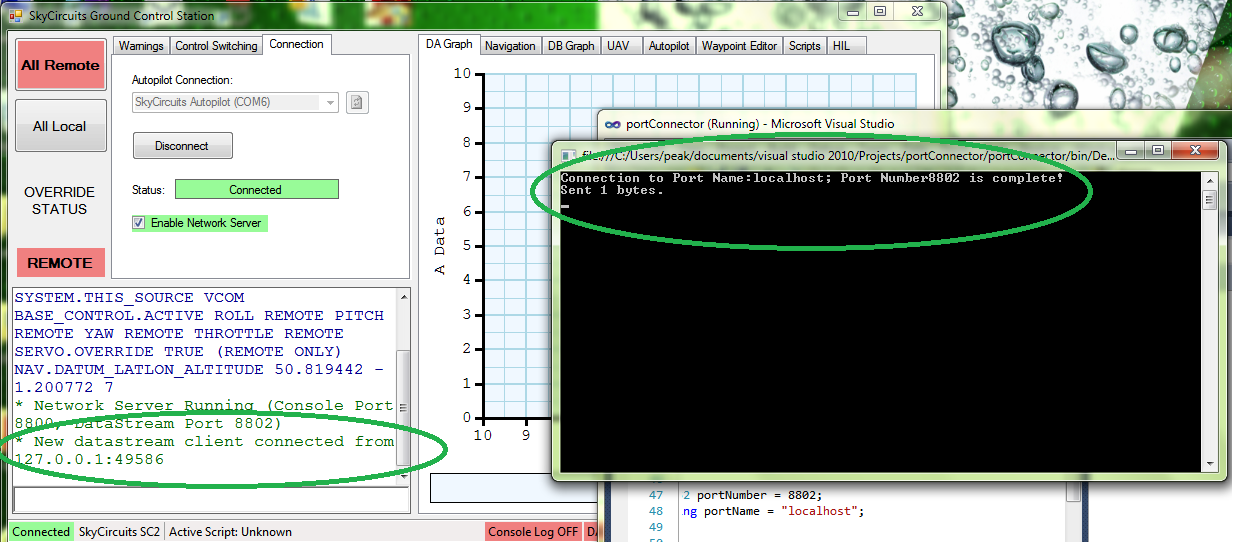
\includegraphics[width=1.00\textwidth]{testing_screenshots/test_sending.png} 
\end{center}
\caption{A screen shot showing the connection with the UAV was successful\label{connect to Stream Port}}
\end{figure}

\subsection{Using Console Application: Testing Connection to UAV, Receive Data from Stream Port}
\label{sec:testing_receive_stream}
Figure \ref{test screenshot} shows a data stream displaying in our test console application.
Firstly, in the GCS program, we write ''da 30 ht''. 
This code makes the height data stream to the ground station, this data then displays on both the graph and in our console application, and we can see the number clearly changes when the height changes.
This is testing that the data stream is working correctly and we have a correct way of getting the data.
Therefore, the Milestone \ref{sec:ms_gs_basestation_comms} is validated.
\begin{figure}[H]
\begin{center}
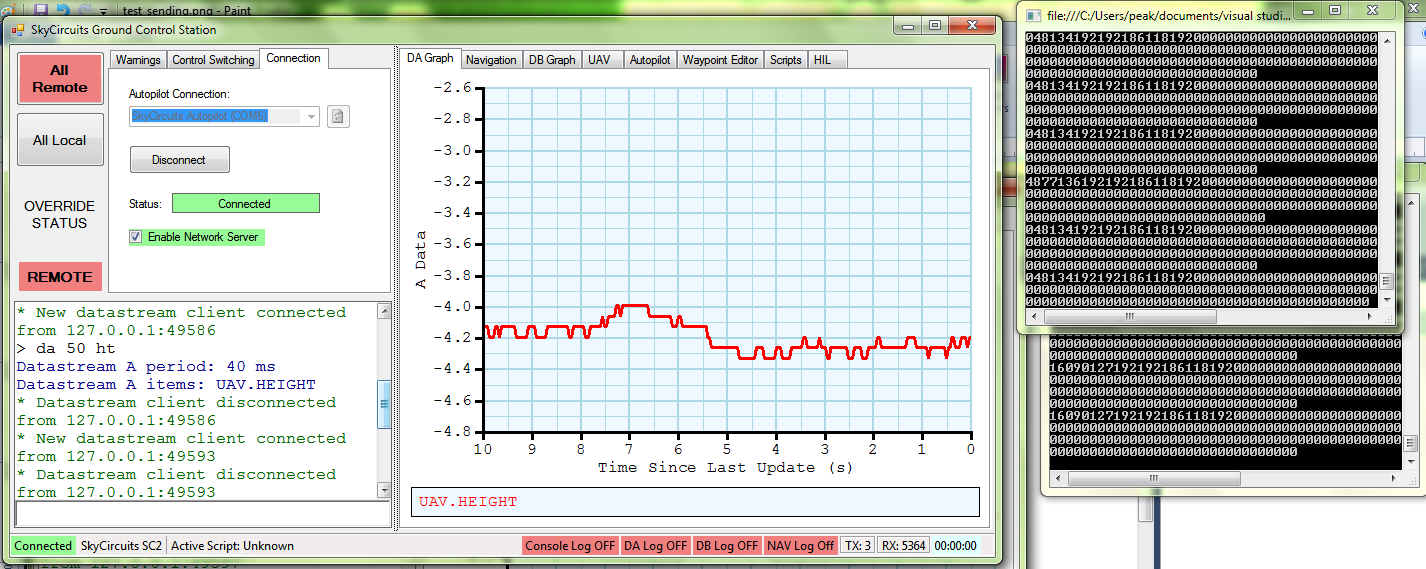
\includegraphics[width=1.00\textwidth]{testing_screenshots/test_data.png} 
\end{center}
\caption{A screen shot shows that the data streams successfully\label{test screenshot}}
\end{figure}

\subsection{Using Console Application: Testing Send Command to Console Port}
\label{sec:send_console}
Figure \ref{test text} shows communication with the console port.
The ground station program allows the user to use the console port to send a string command to it. 
This string command can be tested by the ground station program, which will produce a line with the ''@'' sign on the front of the command sent from the outside of the program.
If the data is correct, the ground station program will detect it and send the data to UAV. 
In the console program, when the user types anything in the console line, it will send byte data to the GCS program.
If the text is a command, the program will process the command and send a byte value as set in the command to the UAV.
The first test is try and type 'hello' into the console line.
The GCS will then see the word 'hello' but there is no command available for it.
Therefore, in the GCS console line, it display 'unknown class HELLO'.
Because we send the word via the console line, there is a \@ sign in front of the 'hello' word in GCS program.
The next line we type in is ''da 50 b''.
GCS software recognises this command, therefore it changes the display in the graph to give information about banking of the UAV.
This test validates Milestone \ref{sec:ms_basic_dummy_server_comms}.
\begin{figure}[H]
\begin{center}
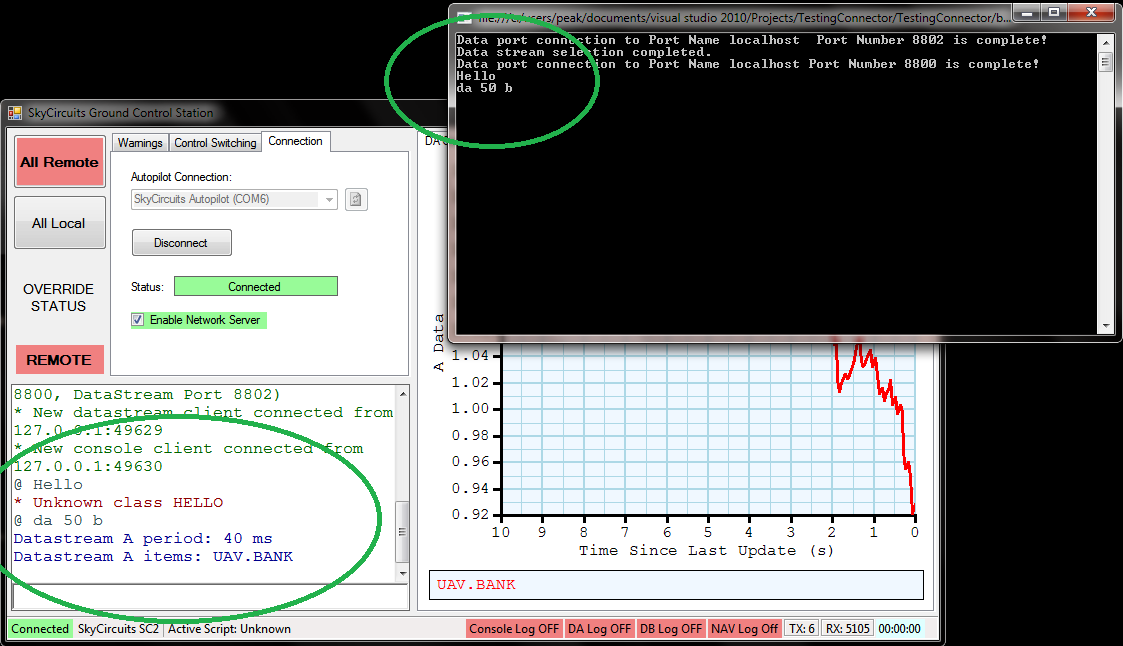
\includegraphics[width=1.00\textwidth]{testing_screenshots/test_sending_test_text_useful.png} 
\end{center}
\caption{A screen shot showing the text sending change the GCS (Ground Control Station) graph value\label{test text}}
\end{figure}

\subsection{Using Window Application: Testing Get Image Button}
\label{sec:test_get_image_button}
The connection between the aircraft and the ground station is using a TCP port, which allows data to be sent from the aircraft in any format. 
In order to test this relationship, a camera will take a picture. 
If the pictureBox displays an image the similar to that expected, the image data is correct.
Figure \ref{camera testing1} shows completed, combined classes together and receiving image data.
This testing combines all the existing methods together in the Window application.
At this point the connector class will be in the main window application.
When the user clicks the 'Get Picture' button on the window application, the program will communicate bidirectionally, sending and receiving that which already stated in section \ref{get image algorithm}. 
From the figure, it clear that the image is downloading and the image has displayed correctly. This test validates Milestone \ref{sec:ms_gs_recieve_image}. 
\begin{figure}[H]
\begin{center}
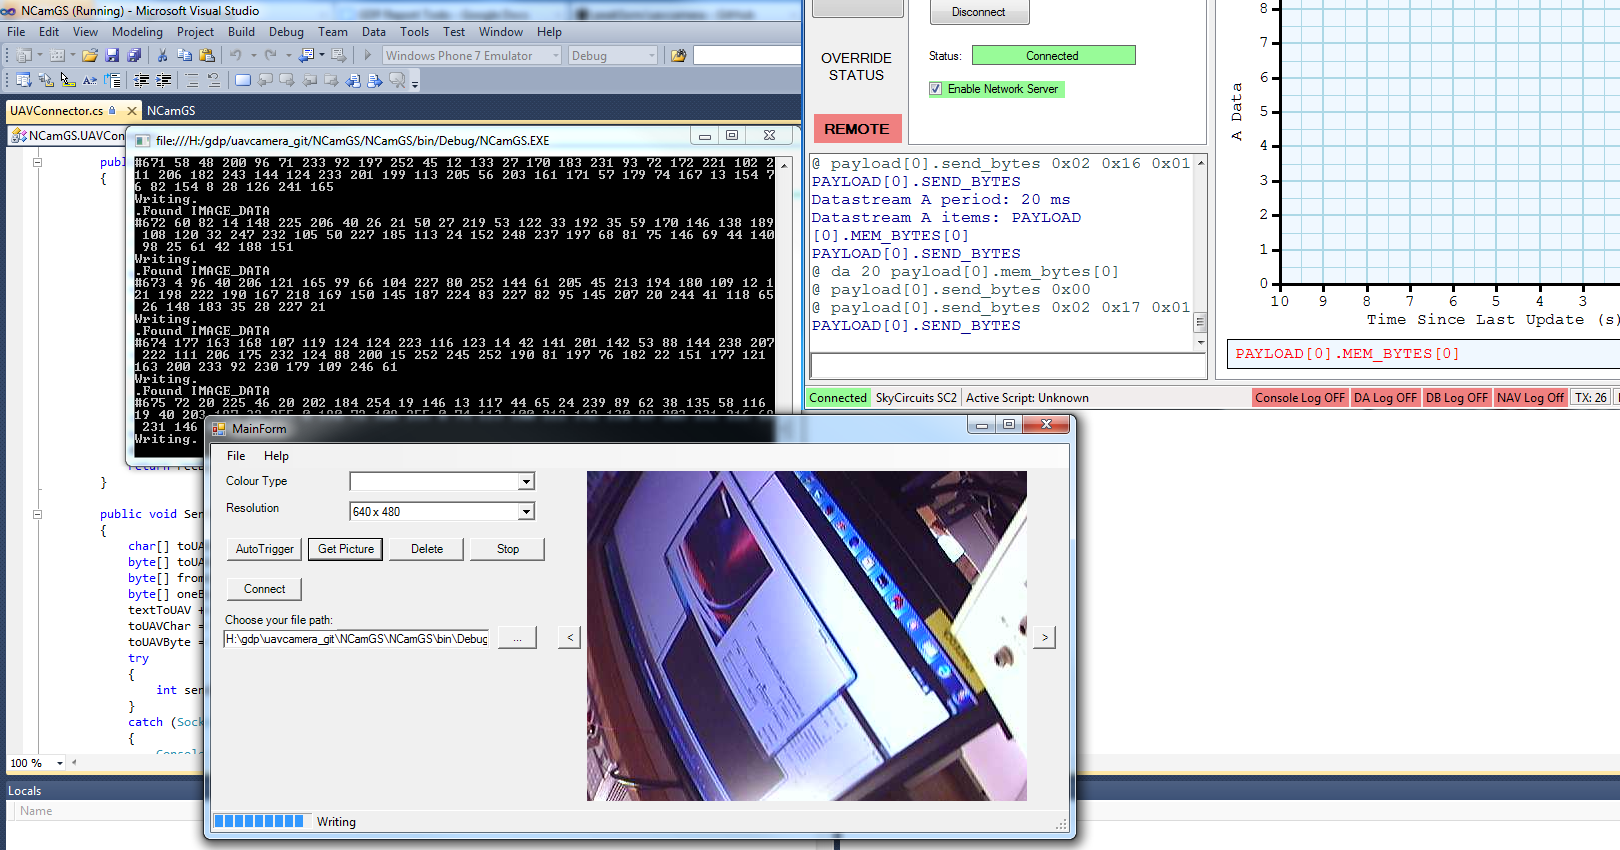
\includegraphics[width=1.00\textwidth]{testing_screenshots/cam_test_11.png} 
\end{center}
\caption{A screen shot showing the picture has been taken correctly\label {camera testing1}}
\end{figure}

\subsection{Using Window Application: Testing Cancel Image}
When the "Cancel" Button is pressed the image stops downloading and is saved in its current state. This test was successful fulfilles specification items \ref{sec:spec_f} and \ref{sec:spec_h}.

\subsection{Using Window Application: Testing Resolution Option}
\label{test_res_op}
When the resolution option changes, the Image viewer program will change the command byte that gets sent to the Console Port of the UAV. 
This can be tested by changing the combo box in the image viewer program and clicking on the Get Picture button.
If it is working correctly, the ground station will see the correct resolution chosen of the picture taken.
Figure \ref{resolution testing} shows a working resolution changing module. 
The PuTTy terminal shows the resolution command that was sent back from the payload.
This proves that the resolution option is working.
This test completes Milestone \ref{sec:ms_pl_img_gs_cam_res}.
\begin{figure}[H]
\begin{center}
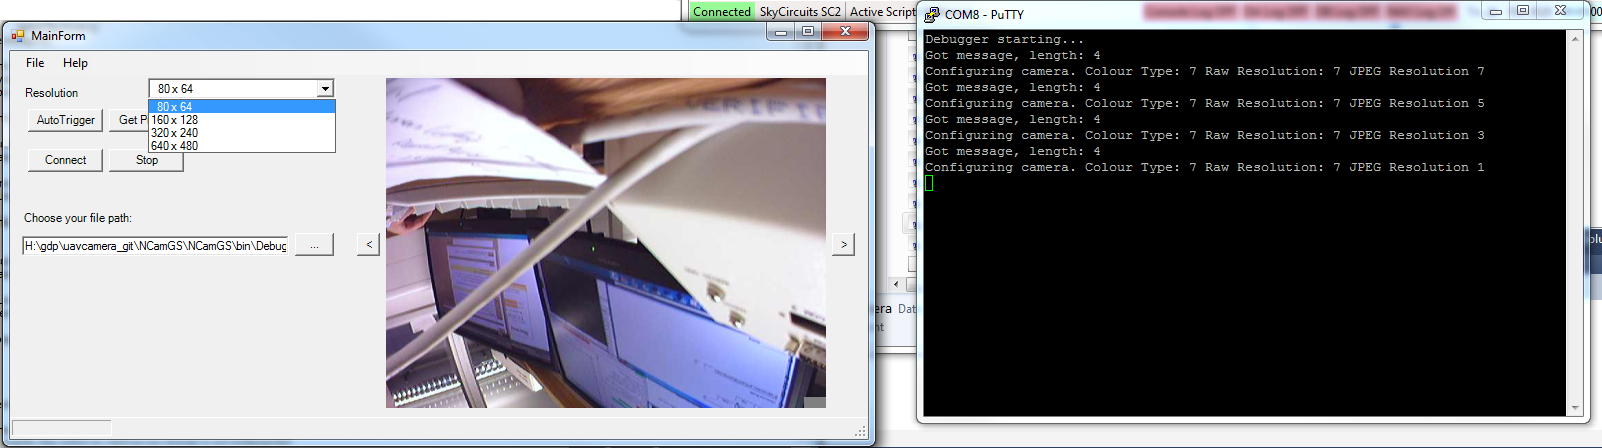
\includegraphics[width=1.00\textwidth]{testing_screenshots/change_res_ncam_1.png} 
\end{center}
\caption{A screen shot showing that a chosen resolution sends different signals to the payload\label{resolution testing}}
\end{figure}

\subsection{Functional User Interface}
\label{func_UI}
The tests listed above verifying Milestone \ref{sec:ms_gs_func_interface} are completed. Figure \ref{completeGUI} shows a complete user interface that is functional and ready for the customer to use.
\begin{figure}[H]
\begin{center}
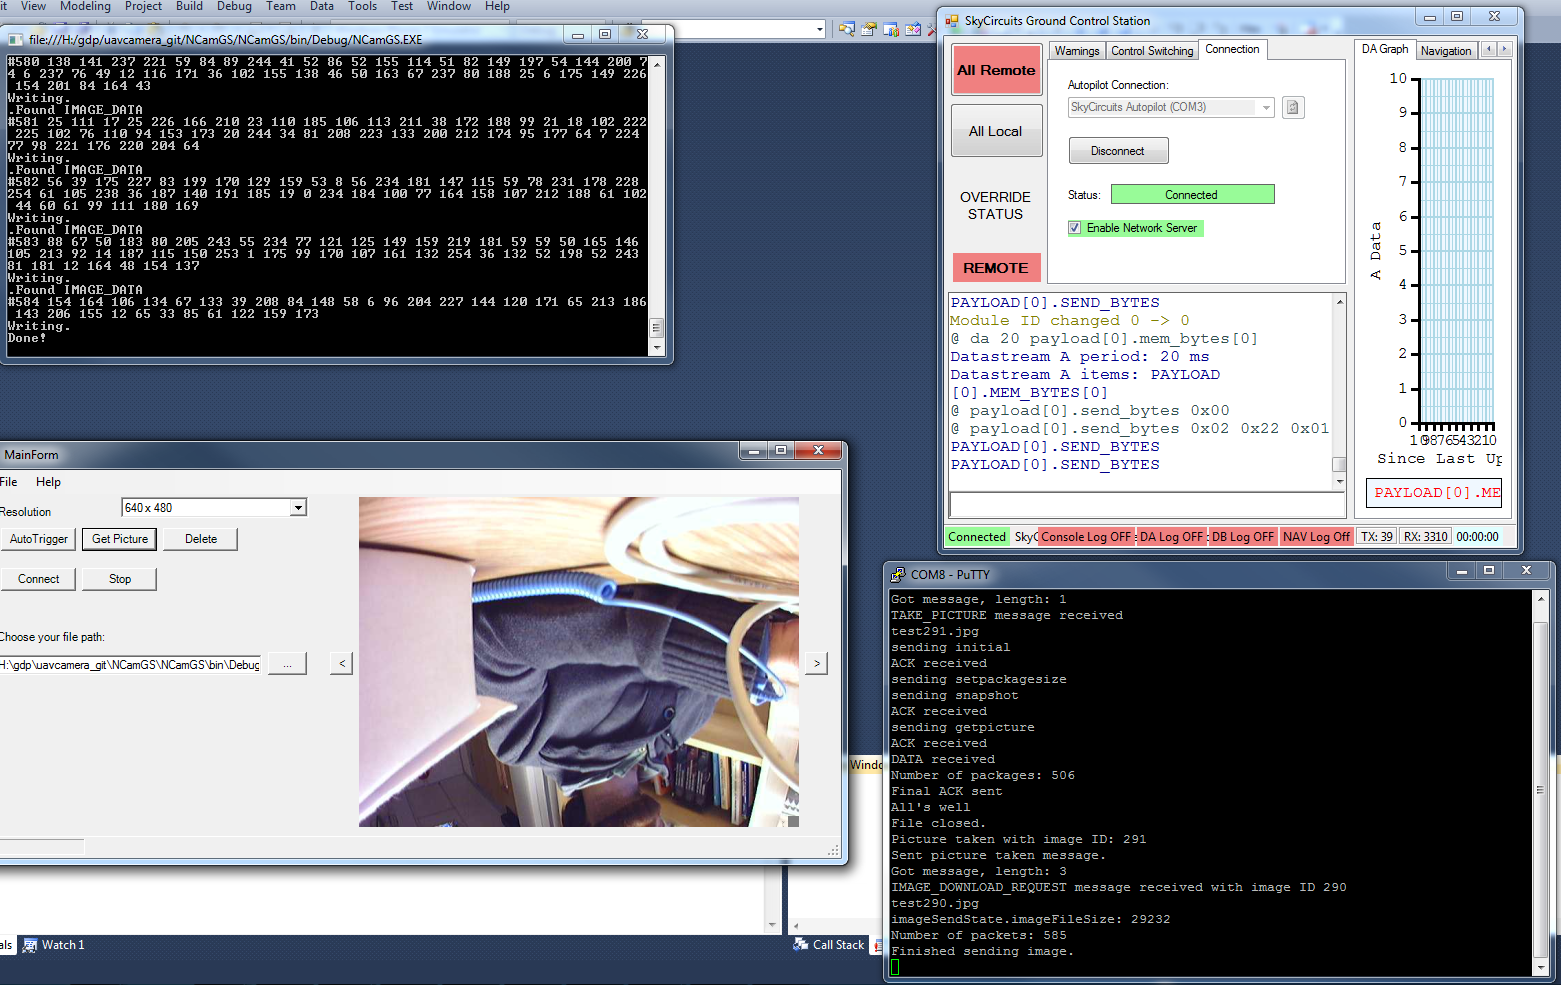
\includegraphics[width=1.00\textwidth]{testing_screenshots/complete_testing_3.png} 
\end{center}
\caption{A screen shot showing a complete UI\label{completeGUI}}
\end{figure}



